%! ~~~ Packages Setup ~~~ 
\documentclass[]{article}


% Math packages
\usepackage[usenames]{color}

% Deisgn
\usepackage{yfonts}
\usepackage{wrapfig}
\font\Cal=cmsy10 at 25pt
\textwidth=.5\textwidth
\def\pstart#1{\noindent\smash{\lower3ex\hbox{\llap{\Huge\frakfamily#1}}}
	\parshape=3 1.5em \dimexpr\hsize-1.5em 2em \dimexpr\hsize-2em 0pt \hsize}
\usepackage[labelfont=bf, labelformat=empty]{caption}
\usepackage[margin=1.4in]{geometry}
\usepackage{multicol}
\usepackage[skip=4pt, indent=20pt]{parskip}
\usepackage[normalem]{ulem}
\usepackage{microtype}
\renewcommand\labelitemi{$\bullet$}
\usepackage{titlesec}
\titleformat{\section}[block]
{\fontsize{15}{15}}
{\dotfill (\thesection)}
{0em}
{\MakeUppercase}
\usepackage{graphicx}
\graphicspath{ {./} }
\pagenumbering{gobble}


% Language Shortcuts
\newcommand\del   {$ \!\! $}
\newcommand\ttt[1]{\en{\footnotesize\texttt{#1}\normalsize}}

\newcommand\npage {\vfil {\hfil \textbf{\textit{המשך בעמוד הבא}}} \hfil \vfil \pagebreak}
\newcommand\ndoc  {\dotfill \\ \vfil {\begin{center} {\textbf{\textit{שחר פרץ, 2024}} \\ \scriptsize \textit{נוצר באמצעות תוכנה חופשית בלבד}} \end{center}} \vfil	}

\newcommand{\rn}[1]{
	\textup{\uppercase\expandafter{\romannumeral#1}}
}

\makeatletter
\newcommand{\skipitems}[1]{
	\addtocounter{\@enumctr}{#1}
}
\makeatother


%! ~~~ Document ~~~

\author{Shahar Perets}
\title{\vspace{-40px}Post reading -- lamb to the slaughter}
\begin{document}
	
	\maketitle
	
	\vfill
		
	\hfil \large Exlusive Report by ``The Onion News": \hfil
	
	\hfil \Large \MakeUppercase{Patrick Maloney was murdered} \normalsize \hfil 
	
	\vspace{2pt}
	\noindent \textit{(Bob Zilman, London, 11.9.1911)}
	\vspace{-8pt}
	
	\begin{multicols}{2}
		\noindent \pstart{Y}esterday, the policeman and detective Patrick Maloney, was found dead in his home by his loyal wife. After she got back from the groccery shop, Mrs. Maloney saw the dead body of her husband thrown away on the floor. Acordding to Jack Noonan, a police detector and a friend of Mr. Maloney, he was hitted by a strong object on the back of his head.
		
		Rumors spread across the country, indicating that the murder weapon could be a metal chain that is being used to tie prisoners to the british prisonships. It's possible that someone was able to rub his chain and free himself. Incidents like that happened several times in the past, though there are no avidence to show that's the case here. In addition, the latest version of the british chain is attached physically to the prisoner's body. 
		
		\begin{wrapfigure}{l}{0pt}
			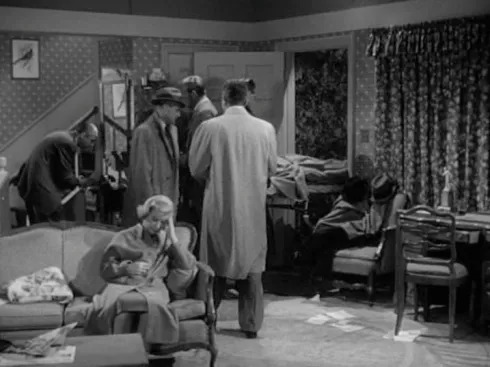
\includegraphics[scale=0.23]{capturfiles_264.jpg}
			\caption[]{The investigation}
		\end{wrapfigure}
		
		\noindent Patrick was known to be able to extract any data out of any scene, and was able to solve some of the greatest mysteries in Great Britany, and was one of the most honored detectives in the London Police Depratmant. As such, he have had several dangerous opponenets--that have come to murder him last night. One of the arrested people, Oliver Jones, was improsined for 20 years till last month, when the jury find him non-guilty. After the fact, it was found that the jury became one of the richest persons in Centeral London. 
		
		Another theory suggest that Patrick was murdered over fights for the inheritage of his father Oliver Molways, who left approximatly half of a million dollars in cash, togather with real estate. Since Mr. Molway is known to be close the jury, he was expected to inhetrite most of the father's propery. 
		
		Mr. Noonan says that ``the police is invastigating the incident, and we have strong avidences condemming Jones as the murder''. When asked about other people that were in the area at the same time, he answered that ``the only known person to be there was Mrs. Maloney, which was validated to be at teh groccer when the murder accured. We're sorry for her loss". 
		
		The funeral will occur next Sunday. His wife and a small represntation of the local police station is expected to come. 
		
		Mr. Noonan refused to answer further questions, and seemed confused about the problem. With that said, he was quite sure Oliver Jones will be convicted. Meanwhile, we remain with many questions about what happend to one of the greatest and bravest detective in Great Britany. 
		
	\end{multicols}
	
	\vfill
	
\end{document}